%------------------------------------------------------------------------------
\chapter{Irregular Sampling}
\vspace{-1cm} \label{cap2}

%\begin{flushright}
%\begin{minipage}{0.7\linewidth}
%\emph{``Quando uma criatura humana desperta para um grande sonho e
%sobre ele lan�a toda a for�a de sua alma, todo o universo conspira a
%seu favor.''}
%\end{minipage}
%\end{flushright}
%
%\begin{flushright}
%{Goethe}
%\end{flushright}

%\vspace{1cm}

%%Colocar uma descri��o do cap�tulo aqui!
%\section{Introdu��o}\label{sec int_cap_2}

In the last chapter, we  reviewed sensor fusion motivations, advantages and techniques. Despite all the growth and benefits from fusing data form multiple sensors, some challenges naturally appear. One of which is related to sampling irregularities introduced in the network.

In this chapter, we review the irregular sampling problem. First, in Section \ref{irregular-sampling} we categorize the different types of irregularities that may occur in sampling and discuss the main causes and its particularities. A diagram is built by categorizing the main types studied in the scientific literature and their causes. Then each irregularity is further discussed, with examples, mathematical models and their subdivisions, where applicable. We end this chapter with a discussion of time synchronization, which is needed to guarantee a common time scale for all nodes in network, enabling the irregularities to be dealt with appropriately.

\section{Introduction}\label{irregular-sampling}

Sampling irregularities may occur due to a variety of issues. Sometimes as undesired side effects of using large sensor networks architectures and others due to deliberate non-uniform sampling schemes. In this section we try to categorize and review the main irregularities observed in practice. The diagram in Figure \ref{fig:diagrama2} provides a simplified overview of them, separated by their sources.

\begin{figure}
\centering
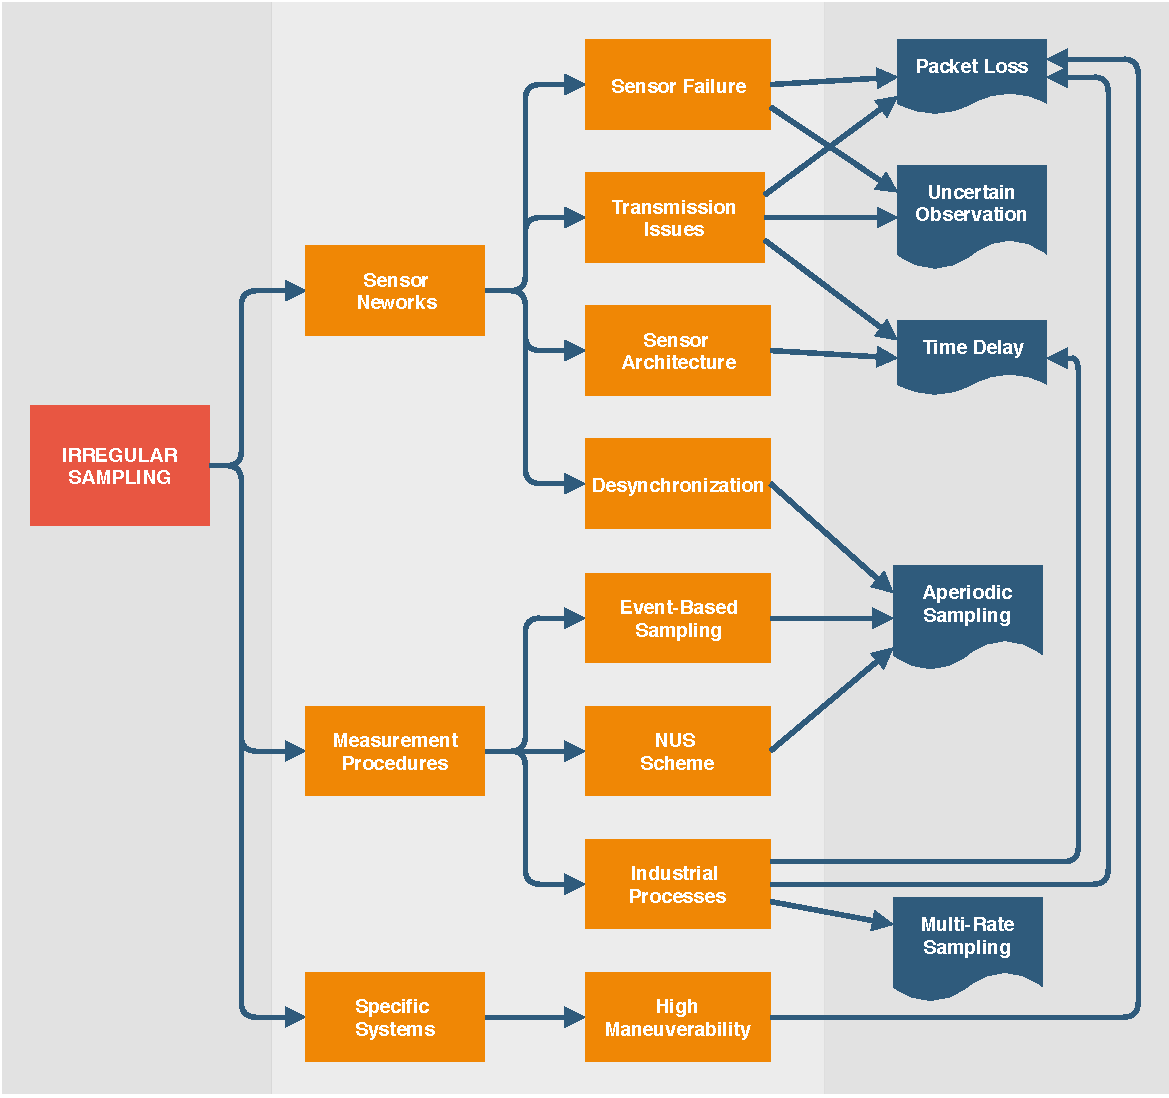
\includegraphics[width=0.9\textwidth]{Imagens/irreg_sampling.pdf}
\caption[Irregular sampling diagram]{Irregular sampling diagram, showing the main causes (in orange) and effects (in blue) of irregularities}
\label{fig:diagrama2}
\end{figure}

Networked system monitoring and control appears to be the main cause of irregular sampling. Unreliable communication channels may lead to random time delays and loss of information, specially if data are transmitted using a common media \citep{Sahebsara2007, Moayedi2011}. In case they get randomly interrupted during transmission or if a sensor fails at some point, the signal received may predominantly contain noise, causing uncertain observation or packet dropouts \citep{Hadidi1979, Wang2009}. Systems that are observed by a large number of desynchronized sensors will provide observations at random time intervals \citep{Micheli2002}. If they are synchronized but designed to operate in a centralized fashion, there is a chance that different time delays are produced due to distinct transmission routes for each sensor \citep{Bar-Shalom2000, Challa2003, Anxi2005}. 

However the communication networks shall not always be held responsible. Some applications are designed to be measured in an irregular way. In event-based schemes, for example, the measurements are transmitted only when certain conditions are met \citep{Liu2014,Zou2017}. Such approach can reduce communication resource consumption substantially \citep{Hu2017}, but will cause aperiodic sampling. Non-Uniform Sampling (NUS) is also intentionally used as an alias detection method \citep{Kunoh2015} or to enhance the spectral resolution of signals, largely used in Nuclear Magnetic Resonance (NMR) spectroscopy analysis \citep{Hyberts2013}. In other situations, due to the nature of the process being observed, the measurement strategy relies on different procedures. A lot of chemical processes, for instance, can be measured in an online, fast rate and delay free fashion, but provides inaccurate data. Therefore, lab analyses are used to improve estimation quality, but they are usually gathered at slower rates, sometimes irregularly and with possible time delays \citep{Fatehi2017}. Other industrial applications suffer from the same dilemma, and the sampling scheme ends up with a multi-rate data transmission, with random time delays and possibly measurement scarcity \citep{Penarrocha2012}. 

Finally, sampling irregularities might also appear due to a specific nature of a system. In some high maneuverable target-tracking applications, for example, there is a chance that the sensor misses the target, transmitting only noise, leading to the so called uncertain observation issue \citep{Wang2009, Chen2013}.

%\duvida{Vale a pena introduzir o assunto de irregularidades do controlador para o atuador (e n�o s� do sensor para o controlador)?}

On the next sections, we review the main irregular sampling effects.

\section{Irregularity Types}
\subsection{Time Delay}

Time-delay systems (TDS) are probably the most common mathematical representation to time delays in practice. The works of \citep{Richard2003, Fridman2014} and the references therein provide a good coverage of the subject. In TDSs, there might be delays in the input or in the output signals, introduced by communication networks, or even in the states themselves. The latter phenomenon is called system with aftereffect or dead-time. Since we are studying the irregular sampling issue, only signal delays are relevant to us.

Considering delays in the measurement model only, \citep{Lu2005} studied the estimation problem when they are constant and known. They describe a linear measurement model as

\begin{equation}\label{eq:delay_model}
	y_i(t)=H_i(t)x(t_i)+v_i(t)
\end{equation}


\noindent
where $i=0,\ 1,\ ...,\ l$ and $l$ is the number of different known delays. $y_i(t) \in \mathbb{R}^{p_i}$ are delayed measurements and $v_i(t) \in \mathbb{R}^{p_i}$ the measurement noises. The known delayed time instants are given by $t_i=t_{i-1}-d_i$, with $d_0=0$, $d_i>0$ for $i>0$ and $t_0=t$. 

For some systems, delays might not be known and constant, but still multiple of a fixed value. In such cases, observations might be received in a burst, when more than one packet arrive between two consecutive sampling instants. When that happens, the estimator might use only the latest measurement and discard all others, or implement a buffer to iterate over all received packets \citep{Moayedi2011}.

However, in many applications the measurements are received by the estimator with irregular and unknown delays. In such cases, time delays can be interpreted as a stochastic process $d(k)$, varying randomly throughout time. \citep{Han2009} describes a discrete-time measurement model for random delayed observations as

\begin{equation}\label{eq:delay_model2}
y(k) = H(k)x(k-d(k))+H(k)v(k)
\end{equation}

\noindent
where $d(k)$ is a random but bounded time delay, assumed to be a discrete-time Markov Chain observable at each sampling time k.

Multiple of a known lag or not, delayed measurements from a multisensor system are subject to arrive disordely, which leads to the sampling irregularity commonly known as to as out-of-sequence-measurements (OOSM). It can be classified in three ways, depending on the number of lags, according to Figure~\ref{fig:oosm}. 

\begin{figure}[!htb]
	\centering
	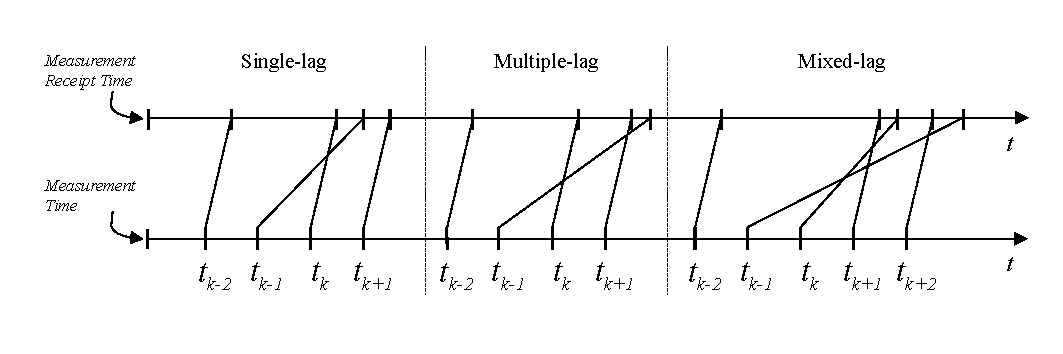
\includegraphics[width=0.75\textwidth]{Imagens/oosm.pdf}
	\caption{Different classes of out-of-sequence measurements irregularities}
	\label{fig:oosm}
\end{figure} 

\citep{Anxi2005} describes four different filtering approaches to deal with OOSM: reprocessing, that stores filter results to rollback with the time-delayed measurement; data buffering, that holds a set of measurements, greater than maximum expected lag, to be sorted before filtering; discarding data, that neglects time-delayed measurements; and directly updating, that uses the delayed information to update current state estimate. \citep{Bar-Shalom2000} used the last approach to describe an optimal filter for the single-lag case.

A summary of causes and effects that time delay causes in an estimator are illustrated in Figure \ref{fig:diagrama_delay}.

\begin{figure}[!htb]
	\centering
	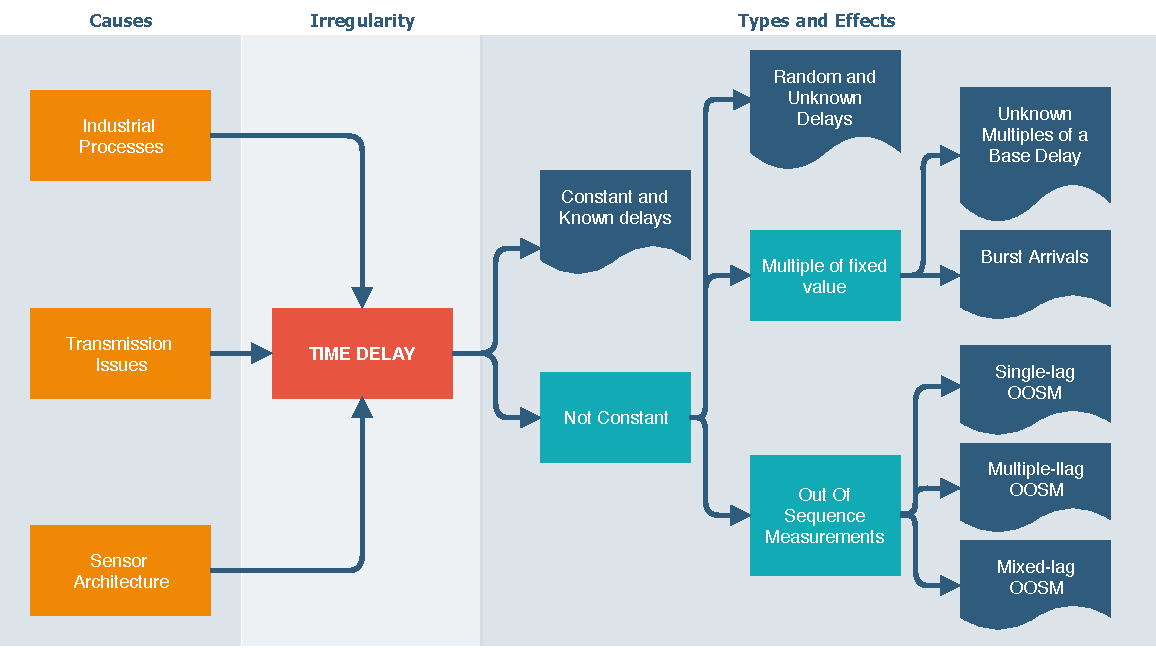
\includegraphics[width=0.75\textwidth]{Imagens/scheme_time-delay.pdf}
	\caption[Time delay diagram]{Time delay diagram, showing the main causes (in orange) and effects (in dark blue) of time delay irregularity. The light blue boxes indicate different types that lead to different effects.}
	\label{fig:diagrama_delay}
\end{figure}

\subsection{Packet Loss}

When data are being transmitted by a large network of sensors, there is a probability they can get lost in the way or they might arrive after a significant delay, which is equivalent to a loss for practical	 applications~\citep{Sinopoli2004}. Usually referred to as packet dropout/loss, missing, intermittent observations or scarse measurements~\citep{Albertos2004} they may happen due to node failures, network congestion, limited bandwidth or temporal failure. 
	
Mathematical description of packet dropouts can be carried out recursively, as described in~\citep{Sun2011}, by

\begin{align}
\centering
\begin{split}
z(t)=H(t)x(t)+v(t), \\
y(t) = \xi(t)z(t)+(1-\xi(t))y(t-1),
\end{split}
\end{align}

\noindent
where $z(t) \in \mathbf{R}^m$ is the measured output transmitted to the estimator, $v(t) \in \mathbf(R)^m$ is white noise, $y(t) \in \mathbf{R}^m$ is the measurement received by the estimator and $\xi(t) \sim Ber(p)$ is a Bernoulli random variable that takes the value 1 with probability $p$ and 0 with probability $1-p$. That is, when $\xi(t)$ is 1, there is no packet dropout. If $\xi(t)$ is 0, however, the latest output is used at current time, in a recursive fashion.

Another way of describing multiple packet dropouts is by limiting the amount of consecutive dropouts ~\citep{ShuliSun2008}, where the received measurements are defined by

\begin{equation}
\begin{split}
y(t) = 	& \xi(t)z(t) + (1-\xi(t))\xi(t-1)z(t-1)+...\\
		& + (1-\xi(t))(1-\xi(t-1))...(1-\xi(t-N+1))z(t-N), N \geq 1,\\
\end{split}
\end{equation}

Such a model dictates that the measurement used by the estimator will be only the most recent available, and the amount of missing observations is limited to $N$. This conclusion can be drawn by the fact that

\begin{equation}
\xi(t)+(1-\xi(t))\xi(t-1) + ... + (1-\xi(t))(1-\xi(t-1))...(1-\xi(t-N+1)) = 1.
\end{equation}

A summary of causes and effects that time delay causes in an estimator are illustrated in Figure \ref{fig:packet_loss}.

\begin{figure}[!htb]
	\centering
	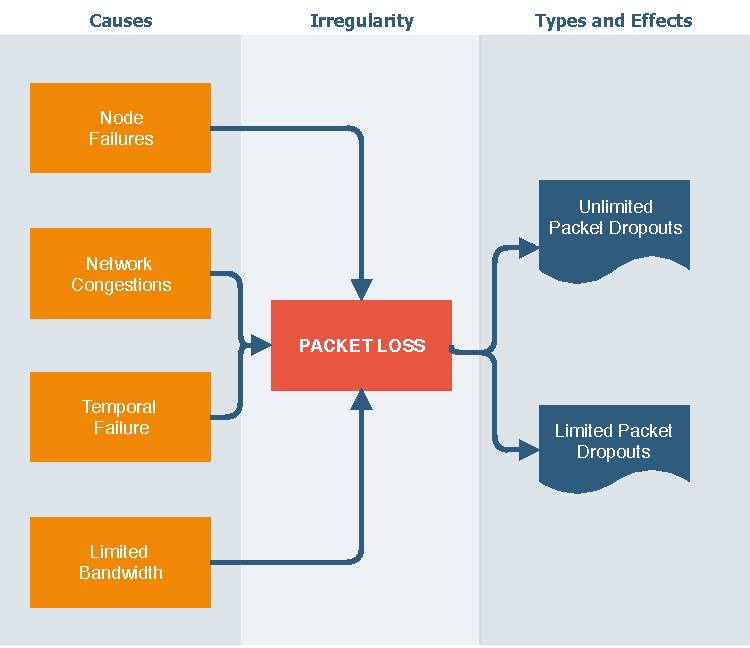
\includegraphics[width=0.75\textwidth]{Imagens/scheme_packet-loss.pdf}
	\caption[Packet loss diagram]{Packet loss diagram, showing the main causes (in orange) and effects (in dark blue) of time delay irregularity.}
	\label{fig:packet_loss}
\end{figure}


\subsection{Uncertain Observation}\label{sec:uncertain}

For some applications, there is a chance that the observation signal sent to the estimator contains only noise. According to \citep{Jaffer1971}, it happens as a consequence of two situations: the observation was taken, but was lost during transmission, due to communication failures; or it was not transmitted at all, as it may happen for target tracking systems, for example, when the object being observed is not tracked at a sample time. An observation model for a sampled-data system can be described as

\begin{equation}
y(k) = \gamma(k)Cx(k) + Dv(k)
\end{equation}

\noindent
where $\gamma(k) \sim Ber(p(k))$ is a Bernoulli random variables, taking values of 0 or 1, with probabilities $p(k)$ and $1 - p(k)$, respectively.

Unlike the packet dropout problem, when the missing data are associated with the total absence of signal, the issue of uncertain observation has to be dealt with differently. A common approach is to detect the existence of signal prior to the assimilation, using a likelihood ratio test.  \citep{Middleton1968} proposes a joint approach to systematically detect and extract information from observation signals. If the estimator and detector are developed separately, te probability of false alarms is not used in the estimator, making it suboptimal. \citep{Nahi1969} developed an optimal recursive estimator, that uses the information of the random variable $\gamma$ in the algorithm, assuming it is independent and identically distributed. \citep{Hadidi1979} generalized the work of Nahi, for the case when the uncertainty of the signals presence is described by a Markovian sequence of binary random variables.

A summary of causes and effects that time delay causes in an estimator are illustrated in Figure \ref{fig:uncertain}.

\begin{figure}[!htb]
	\centering
	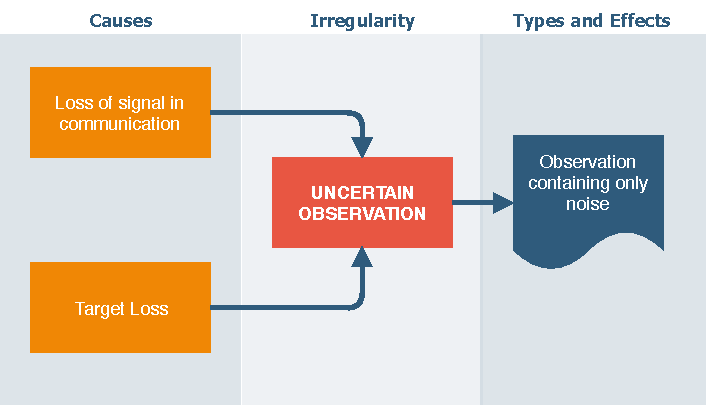
\includegraphics[width=0.75\textwidth]{Imagens/scheme_uncertain.pdf}
	\caption[Uncertain observations diagram]{Uncertain observations diagram, showing the main causes (in orange) and effects (in dark blue) of time delay irregularity.}
	\label{fig:uncertain}
\end{figure}

\subsection{Aperiodic Sampling}\label{sec:aperiodic}
	
All irregularities discussed so far may be present even in a periodic sampling scheme. However, for some applications, the sampling intervals are time-varying due to a variety of phenomena, causing what is called as aperiodic or asynchronous sampling. It can be the case of networked and embedded control systems, with unpredictable networked-induced issues, like irregular faults on samplers, oscillated loads, intermittent saturation or even variations in system components or parameters \citep{Shen2016}. Some imperfections may cause what is known as sampling jitter noise, which leads to time intervals being almost uniform. Automotive applications, radar imaging or event controlled systems are a few examples. In them, jitter noise happens due to sampling frequency similar to clock frequency, sampling requests delayed by the network or imperfect synchronization \citep{Eng2005}. For networks with a large amount of unsynchronized sensors, measurement arrival time intervals are randomly spaced and can be modeled as a stochastic process \citep{Micheli2002}. 

Sometimes, the system being observed has particularities that causes the aperiodic sampling. One example is seismology, where the spatial coordinates are irregularly sampled, because of natural obstacles \citep{Marvasti2001}. Other large scale systems, such as power grids, have sensors with a huge geographical separations, and different communication links to the estimation hub, which causes multiple and random inter-observation intervals \citep{Yan2017}.

Whereas for most cases, the non-uniformities in sampling time intervals appear as unwanted effects, there are cases when the sampling rule is designed to work irregularly. If there are limitations of communication resources (limited bandwidth or computation capacity) or a need for a reduced energy consumption, for example, time-driven sampling might be neglected in favor of an event-based scheme. In such strategy, an event-triggering mechanism is responsible for determining the sampling instants, according to Figure~\ref{fig:event-based}. For time-driven schemes, a clock triggers the transmission instants (a), while event-driven sampling instants depends on the sensor output itself with an optional feedback loop from the estimator, to assess estimation performance. Therefore, the trigger mechanism design provides a trade-off between performance and resource consumption efficiency, attracting a lot of research interest \citep{Liu2014}. The most common strategy for event-driven state estimation is the send-on-delta (SOD) \citep{Miskowicz2006}, which triggers the transmission when the value of the measured state deviates from the previous assimilated observation by an interval $\pm \Delta$, with $\Delta>0$. Other strategies were studied in \citep{Zou2017}. To avoid the risk of unexpected high amount of triggered measurements in a short period of time, which can lead to the dreaded Zeno behavior \citep{Tabuada2007}, lower-bounds can be defined both for the $\Delta$ value or for some explicit minimum inter-event time. 

\begin{figure}[!htb]
	\centering
	\begin{subfigure}
		\centering
		\text{(a)}\\
		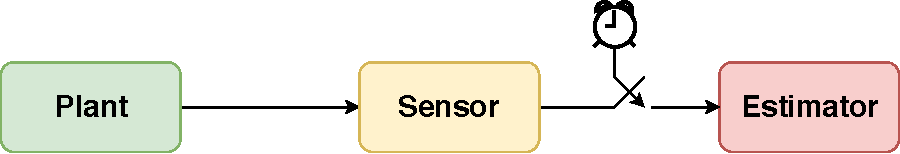
\includegraphics[width=0.75\textwidth]{Imagens/Event-based_clock.pdf}	
		\label{fig:evtb1}
	\end{subfigure}
	\vspace{1cm}\\
	\begin{subfigure}
		\centering
		\text{(b)}\\
		\vspace{0.25cm}
		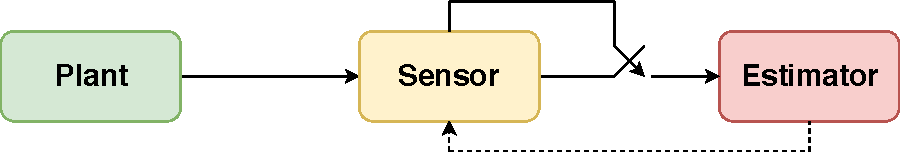
\includegraphics[width=0.75\textwidth]{Imagens/Event-based.pdf}
		%		\caption{}
		\label{fig:evtb2}
	\end{subfigure}
	\caption[Time-driven and event-driven sampling schemes]{Time-driven (a) and event-driven (b) sampling schemes. The connection between sensor and estimator is triggered by different mechanisms.}
	\label{fig:event-based}
\end{figure}

The measurement model of a linear system with aperiodic sampling can be defined as

\begin{equation}\label{eq:aperiodic}
y(t_k) = H(t_k)x(t_k) + v(t_k)
\end{equation}

\noindent
where $t_k$ is the random sampling time instant and the observation model matrix $H(t_k)$ is time-varying, if derived from the discretization of a continuous time system.

Generalizations of aperiodic sampling can be divided in two categories, based on how the estimator perceives the irregularity: as time noise added to a periodic pattern; or as a stochastic process, according to Figure~\ref{fig:aper-samp}. 

\begin{figure}[!htb]
	\centering
	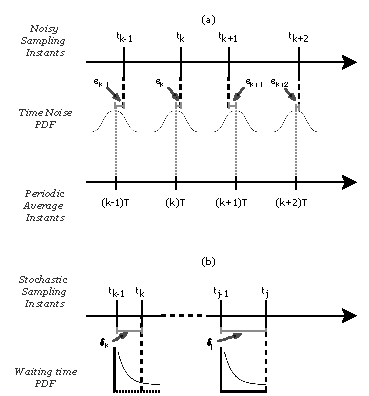
\includegraphics[width=0.85\textwidth]{Imagens/noisy_stoch_samp.pdf}	
	\caption[Aperiodic sampling categories]{Aperiodic sampling categories: (a) noisy sampling over periodic intervals, with a Gaussian random variable added to expected time instants $kT$; and (b) sampling instants modeled as a stochastic process, with time intervals characterized by an exponential random variable (cumulative distribution functions are shown, for different $\lambda$ parameter values.)}
	\label{fig:aper-samp}
\end{figure}

For the first case, random time instants $t_k$ and the random time intervals $\delta_k$ can be defined as:

\begin{equation}
\begin{split}
t_k & \triangleq kT + \epsilon_k, \\
\delta_k & \triangleq t_k - t_{k-1} 
\end{split}
\end{equation}

\noindent
where $t_k$ is the k\textsuperscript{th} sampling instant, $T$ is the periodic time interval and $\epsilon_k$ is the deviation from the expected value $kT$. Note that, if the sampling time instants are a sequence of i.i.d Gaussian random variables, with variance $\sigma^2$, that is $t_k \sim \mathcal{N} (kT, \sigma^2)$, $\forall k \sim \mathbb{N}$, then the time interval random variable is Gaussian, with expected value $T$ and variance $2\sigma^2$, that is $\delta_k \sim \mathcal{N}(T,2\sigma^2)$.

For the stochastic process generalization, sampling time instants $t_k$ can be defined by the random time intervals $\delta_k$, such as:

\begin{equation}
\begin{split}
\delta_k & \triangleq t_k - t_{k-1}, \\
\delta_0 & \triangleq t_1
\end{split}
\end{equation}

\noindent
where random time intervals $\delta_k$ can be modeled, in the most flexible way, as a gamma probability density function, that is $\delta_k \sim \Gamma(k,\theta)$. If the shape parameter $k$ is a positive integer, it becomes an Erlang distribution, as used in \citep{Kanchanaharuthai2002}. For the most common case, where $k$ is held constant, the random time interval $\delta_k$ follows an exponential pdf the time sequence $t_k$ is represented by a Poisson stochastic process \citep{Micheli2002}.

A summary of causes and effects that time delay causes in an estimator are illustrated in Figure \ref{fig:aperiodic}.

\begin{figure}[!htb]
	\centering
	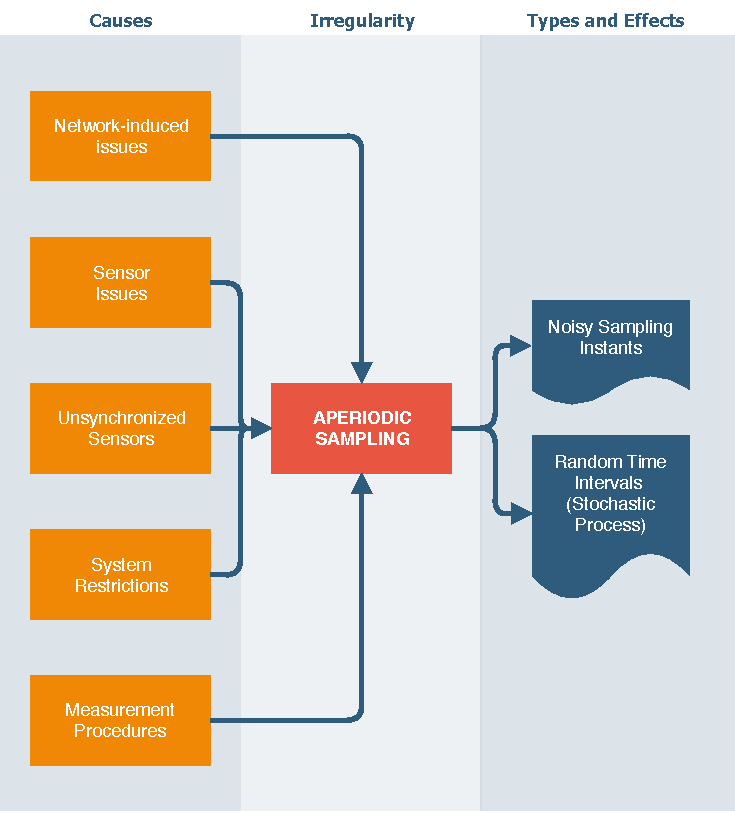
\includegraphics[width=0.75\textwidth]{Imagens/scheme_aperiodic.pdf}
	\caption[Uncertain observations diagram]{Uncertain observations diagram, showing the main causes (in orange) and effects (in dark blue) of time delay irregularity.}
	\label{fig:aperiodic}
\end{figure}

\subsection{Multi-Rate Sampling}

The last irregularity discussed is the multi-rate sampling. Generally, it refers to multiple sensors measuring the same system at different sampling rates. Many industrial processes need to control challenging variables that can be measured by online instruments that provide regular, fast rate and delay free information, but with low precision. Therefore, more accurate data are needed and usually available after slow and irregular laboratory analysis \citep{Penarrocha2012, Fatehi2017}. The combination of both sources of measurements leads to a multi-rate sampling scenario. 

A more common approach is the use of various sensors measuring the same physical information, to obtain better estimates, which has been drawing attention from real world applications, such as target tracking, robotics, surveillance and military. For such strategy, the sampling rates perceived by the estimator are often different from one another. The work of \citep{Lin2016} and the references therein provide a wide coverage of scenarios derived from multi-sensor multi-rate systems. 

Figure \ref{fig:multi-rate} illustrates the ways multi-rate sampling can manifest in a system. The different rates from the various sensor devices can be periodic (a), aperiodic (b) or even a mixture of both, as is the case for most industrial applications with laboratory analysis.

\begin{figure}[!htb]
	\centering
	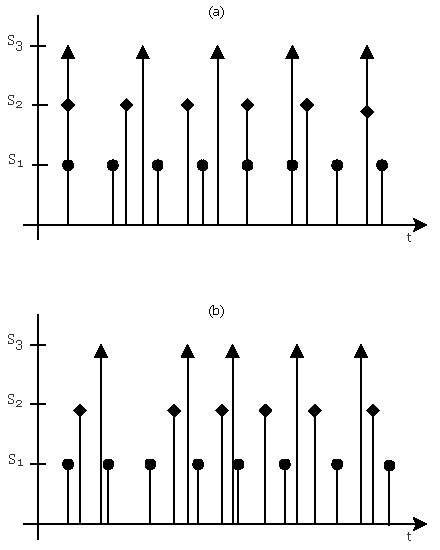
\includegraphics[width=0.5\textwidth]{Imagens/multi_rate.pdf}	
	\caption[Periodic and aperiodic multi-rate sampling scheme]{(a) Periodic and (b) aperiodic multi-rate sampling scheme.}
	\label{fig:multi-rate}
\end{figure}

Aperiodic sampling rates can be described the same way as in Section \ref{sec:aperiodic}, by equation \ref{eq:aperiodic}. Periodic multi-rate measurements can be modeled as

\begin{equation}
	y_i(k_i) = H_i(x(k_i)) + v_i(k_1)
\end{equation}

\noindent
where $y_i(k_i)$ represents the $k_i^{th}$ observation from sensor $i$ and $H_i$ is the discrete measurement model matrix.

A summary of causes and effects that time delay causes in an estimator are illustrated in Figure \ref{fig:multi_rate}.

\begin{figure}[H]
	\centering
	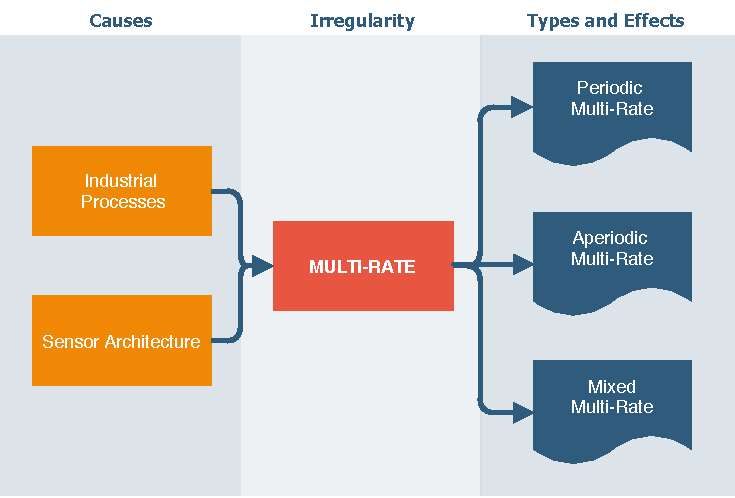
\includegraphics[width=0.75\textwidth]{Imagens/scheme_multi-rate.pdf}
	\caption[Uncertain observations diagram]{Uncertain observations diagram, showing the main causes (in orange) and effects (in dark blue) of time delay irregularity.}
	\label{fig:multi_rate}
\end{figure}


\section{Time Synchronization}

Most of the issues are due to sensor networks or architecture. Sensor fusion without synchronization introduces unknown or uncertain timestamp. They happen because blablabla

Explain how sensor clock words

Multi-sensor fusion require the knowledge of measurement timestamp. Julier proved the impact on not knowing. One can synchronize via several techniques or use other approaches, like PDAF, CU, etc.





\citep{Sivrikaya2004}
Time synchronization is an important issue in multihop, ad-hoc wireless networks such as sensor
networks. Many applications of sensor networks need local clocks of sensor nodes to be synchronized, requiring various degrees of precision. Some intrinsic properties of sensor networks such as limited resources of energy, storage, computation, and bandwidth, combined with potentially high density of nodes make traditional synchronization methods unsuitable for these networks. Hence there has been an increasing research focus on designing synchronization algorithms specifically for sensor networks.



\citep{Brahmi2013}
The sensor-related time delay and the trend towards multi-sensor data fusion require to know the exact measurement timestamps in order to properly interpret the sensor data and therefore enhance the performance of the environmental perception algorithms by performing an optimal sensor data fusion. Furthermore, the evaluation of the perception sensors, by comparing their measurements to those of a ground- truth system, requires a correct timestamping; otherwise, measurement deviations will be erroneously interpreted as a bad accuracy of the sensor. Therefore, different methods and tools were developed to analyze the time delay and the timestamp of different environmental perception sensors



\citep{Ping2003}
Network time or time synchronization is essential for any communications networks, especially for wireless sensor networks. For example, data collected by sensors need global time stamps.

NTP --- The Time Synchronization Scheme for Internet
The time synchronization scheme widely adopted in traditional computer networks is the Network Time Protocol, NTP [13] [14]. A NTP client synchronizes its time with a NTP server using the server?s time provided in a NTP packet and one half of the measured round trip time. In this way a NTP client can be synchronized within a few milliseconds error.
However, we argue that two-way time synchronization techniques, including NTP are not suitable in wireless sensor networks. The basic assumption of a two-way time synchronization method is that the time transfer path is reciproca

Elson proposed a Reference broadcasting synchronization technique [6][7][8]
for wireless sensor networks. In RBS, a reference message
is broadcasted. The receivers record their local time when
receiving the reference broadcast, and then they exchange their recorded time. In this way, they have the knowledge of their time offset with each other. When each mote takes the average of its time offsets to all other nodes that have observed the same reference, a relative network time is achieved among all the receivers.

DMTS
Having studied NTP and RBS, we felt the need to develop a more suitable time synchronization technique that avoids round trip time estimation, synchronizes sender and multiple receivers at the same time and require less number of message transfers than RBS. Other design considerations are scalability, energy consumption, computation cost and user application support.


\citep{Huck2011}
unknown latencies pose a problem in data association and temporal synchronization. Consequently, a method to estimate or incorporate the latencies is needed in all sensor fusion algorithms in order to derive the real time of a measurement.
The crucial first part of every sensor data fusion is the data association, including the temporal synchronization of measurements from different sensors. The exact time at which the measurement was taken is needed. Unfortunately, not all sensors provide such information

Hence, the earliest timestamp available for a radar measurement is the time of arrival at a data acquisition system, where this measurement data is processed



Y. Bar-Shalom related to Probabilistic Data Association Filters (PDAF). 




\citep{Kwok2004}
. In many real-time applications of particle filters, how- ever, sensor information arrives at a significantly higher rate than the update rate ofthe filter. The prevalent approach to dealing with such situations is to update the particle filter as often as possible and to discard sensor information that cannot be processed in time. In this paper we present real-time particle filters, which make use of all sensor information even when the filter update rate is below the update rate of the sensors.
How can we deal with situations in which the rate of incoming sensor data is higher than the update rate of the particle filter?
Instead of discarding sensor readings, we distribute the samples among the different observations arriving during a filter update	


\citep{Julier2005}
However, all of the methods assume that, although
the measurements are delayed (by a potentially random amount), the amount of delay is known. However, situations can arise in which the time delay is not known perfectly. Possible reasons include:
1) Observations are time stamped when they become available to the filter, not when the observation was taken. One example of this is image acquisition using consumer-grade hardware such as a webcamera. Each image acquired by the camera is not time stamped when the image was taken. Rather, the image is time stamped when the data becomes available to an image processing application. Because of non deterministic OS delays (due to buffering, context switches and the like), the latency between acquiring an image and making it available is known imperfectly.
2) Observations are time stamped from a local clock without centralized clock synchronization. In this case, there will always be deviations between clocks at different nodes and, as a result, latency cannot be calculated by subtracting the observation time from the current filter time
Even though the latency is unknown, it might be possible
to statistically characterize it through experimentation1.In this paper we assume that the latency is quantized and is bounded by known values
The uncertainty of the delay was also resolved by means of Probabilistic Data Association Filter (PDAF).
Julier and Uhlmann [6] suggested a method in which
an unknown time delay could be treated by means of the covariance union algorithm. In this method, the covariance was estimated conservatively since the worst case, unknown delay, was considered. But, if the time delay is able to be modeled as a form of a distribution, it is helpful in estimation using that quantity considering the uncertainty of the delayed time.


\section{Chapter Summary}

In this chapter, the main sampling irregularities are reviewed: time delay, packet loss, uncertain observation, aperiodic sampling and multi-rate sampling. Diagrams describing their causes, types and effects were built for each of them. We also describe the necessary modifications to the observation models of state estimation. 

For the simulated systems of this work, aperiodic sampling with time delay was chosen, since it describes a more general irregularity.

\clearpage